\documentclass[12pt]{article}

\usepackage{setspace}
\usepackage{hyperref}
\usepackage{graphicx}
\usepackage{url}
\usepackage{xcolor}
\newcommand\todo[1]{\textcolor{red}{#1}}

\onehalfspacing

\parskip=2ex
\parindent=2em

\title{SWEN439 Visualisation Essay \\ John Snow's Cholera Map}
\author{Hai Tran 300224467}
\date{\today}

\begin{document}
\maketitle 

%Optional abstract
\begin{abstract}

\end{abstract}
\textcolor{red}{
You will pick a visualisation and write an essay about that visualisation. 
You can do the cholera map, then show other things that were similar at the time, and for future show what visualisations came after that resemble it. Like dot maps. They would be not the main topic, but just an example of modern visualisations that are similar or you can contrast it with modern visualisations for disease spread to show how we do the same thing these days but use perhaps different visualisations.
}

\begin{itemize}
\item A clear description of the visualisation and how to read / interpret it
\item What questions does this visualisation address effectively and which does it not?
\item Is this a visualisation that is easy to use for novice viewers, or is it more intended for experts?
\item What is the history of the visualisation? Where did it come from? Where is / was it used?
\item What is the current state of research with respect to this visualisation?
\end{itemize}

\section{Introduction}

\section{The History of John Snow's Cholera Map}

In the nineteenth century, thousands of lives had been lost due to a disease called cholera. Although unknown at the time, cholera is caused by a bacteria called Vibrio cholerae, doubling in number every thirteen minutes and attacking the stomach and intestines \cite{channel1}. This can provoke severe vomiting and diarrhea in victims, eventually causing an agonizing death to the victim in a matter of hours \cite{heros, channel1}. During the time of the nineteenth century, there was no cure for cholera and no one knew what caused the disease. Doctors were convinced cholera was contracted through miasma: harmful airborne odours emanating from decaying waste, repulsive water or soil \cite{test}. This theory was based on observations that showed poor areas being more susceptible to cholera, deaths in these regions occurring frequently \cite{heros}. However, a physician by the name of John Snow had an opposing view. Snow contested the idea of cholera being caused by miasma, instead, hypothesising that cholera was a waterborne disease. In particular, Snow believed that cholera may be in the water supply contiminating the water. Snow came to this hypothesis after previously studying various outbreaks of cholera, writing academic papers that discussed his findings, yet no one believed him \cite{original}. 

During the nineteenth century, 2.5 million people were estimated to be living in London. It was the largest city that had been built and contained the largest population at the time \cite{channel1, tedtalk}. An estimated third of the population lived in slums, up to 8 in a room, and up to 40 to a house. Due to such a large population, this provoked filthy and unsanitary living conditions. People had cesspools containing fecal matter in their basements, eventually accumulating overtime. All this supported the idea that cholera was caused by miasma and unpleasant smells caused from these living conditions. In an attempt to mitigate the smell and prevent cholera, authorities created a law that made citizens empty their cesspools in the Thames river. This action led to contamination of the water supply, leading to a cholera outbreak \cite{tedtalk, johnson}. 

On 28th of August, 1854, a cholera epidemic had broken out in the Soho district of London, England \cite{tedtalk}. After 3 days, 127 were found dead in London due to the epidemic. Within a few weeks, 600 were estimated dead \cite{youtube, tedtalk}. Snow lived in the Soho district near the cholera outbreak and wanted to investigate his hypothesis of cholera being spread through water. He suspected that if his hypothesis were true, incidents of the disease would involve a single source that everyone was going to, incidents of cholera clustering around the source of contamination such as a particular water pump \cite{test, tedtalk, johnson}. 

Snow tested his hypothesis by interviewing locals about cases relating to cholera with the help of Reverend Henry Whitehead. \todo{introduce whitehead} Since Reverend Whitehead was socially connected and knew most of the locals, Snow was able to track down most cases of cholera with the help of Whitehead \cite{tedtalk}. Snow searched for patterns, analysing data collected from the interviews, asking locals whether they knew if the victims had drunk from a particular water source, or whether they had not. He found increasingly that people who drank from a particular water pump were getting sick, and people who did not, were not getting sick. He also found that a brewery located near this pump had an independent water source where workers were not contracting the disease \cite{blog}. Snow found that the brewery workers were drinking beer rather than water which further supported his hypothesis \cite{youtube}.

Snow thought of representing this data as statistics in a table, but eventually had the thought to do a visualisation which provided a high level view of the statistical information that he wanted to display \cite{tedtalk}. Snow plotted data on a map containing water pumps, and every death from cholera that he had collected to see if there was a pattern. He found that 578 deaths had occurred in a small neighbourhood, near a particular water pump on Broad street \cite{channel1}. Thousands of people lived near the Broad street pump, most use it as a water supply to drink from. However, he noticed outliers from the information he collected where a victim by the name of Susanna Eley had contracted cholera but lived far away from the broad street pump. With further investigation, Snow found out that Eley's mother had moved from Broad street and preferred the water in which her son sent her a daily supply from the broad street pump. This evidence supported Snow's hypothesis and could not be ignored by the local authorities \cite{channel1}. 

Statisical analysis of the data collected and the visualisation led Snow to track the origin of the outbreak in the Soho district to the Broad Street water pump. Snow notified the authorities to decommission the pump in Broad street immediately \cite{test}. Only 3 ft away from the pump was an open sewer. Because of the close proximity, sewerage had leaked into the water supply through crevices and cracks. 

On the 8th of September 1854, the water pump handle from Broad street was removed due to the evidence Snow provided to the authorities \cite{youtube}. Coincidently, the cholera outbreak stops. Although Snow had the pump handle removed, the cholera epidemic had already been on the decline. It is not certain that removing the handle stopped the outbreak, as opposed to the outbreak burning itself out. 

By 1896, when the next cholera outbreak had broken out, authorities had been successfully convinced by John Snow's map, and warned everyone to start boiling their water. This was ``the last time that London had seen a cholera outbreak since" \cite{tedtalk}.

John Snow's method of mapping statistic data to create a visualisation of the spread of the disease is still used today \cite{channel1}. 

\section{John Snow's Cholera Map}

John Snow's cholera map was based in the Soho distrinct in London, hand drawn by Snow himself. It was a bird's eye view of neighbourhoods in the district containing information about cases that he had collected from the cholera outbreak. Since Snow was particulary interested in whether cholera was a waterborne disease, he decided to draw black cricles that showed locations of each water pump in his map. Next to the image, he labelled on the map ``PUMP" in capitialized text. Snow plotted each case of cholera on the map, drawing thin black strokes which formed horizontal bars. Each bar represented a death in the neighbourhood caused by cholera \cite{tedtalk}.


The map could be considered a spot map or a dot map. 



On it, thin, tiny strokes represent deaths and circles show the locations of water pumps. The message of the map is clear: Deaths cluster around the Broad Street well, which had been poisoned by fecal matter from a sick baby (this was discovered later). John Snow not only drew the map, but he also convinced the local authorities to remove the handle of the water pump, an action that stopped the outbreak. Snow, many have said, changed medicine forever. \cite{heros}

Each black bar represented a death in the neighbourhood \cite{tedtalk}. As you get further away from the pump, the deaths seem to get less and less frequent. So you can see something poisonous emanating out of this pump on the map. 

The deaths at each address are indicated by the little horizontal lines, stacked up from the street like a pile of little corpses. Snow has made the map big enough to include the locations of the other water pumps in the vicinity, clearly showing a drop-off in cholera deaths where houses are nearer to a different pump. Visualizing his data allowed Snow to investigate abnormalities in the outbreak. \cite{blog}

\begin{figure}
\centering
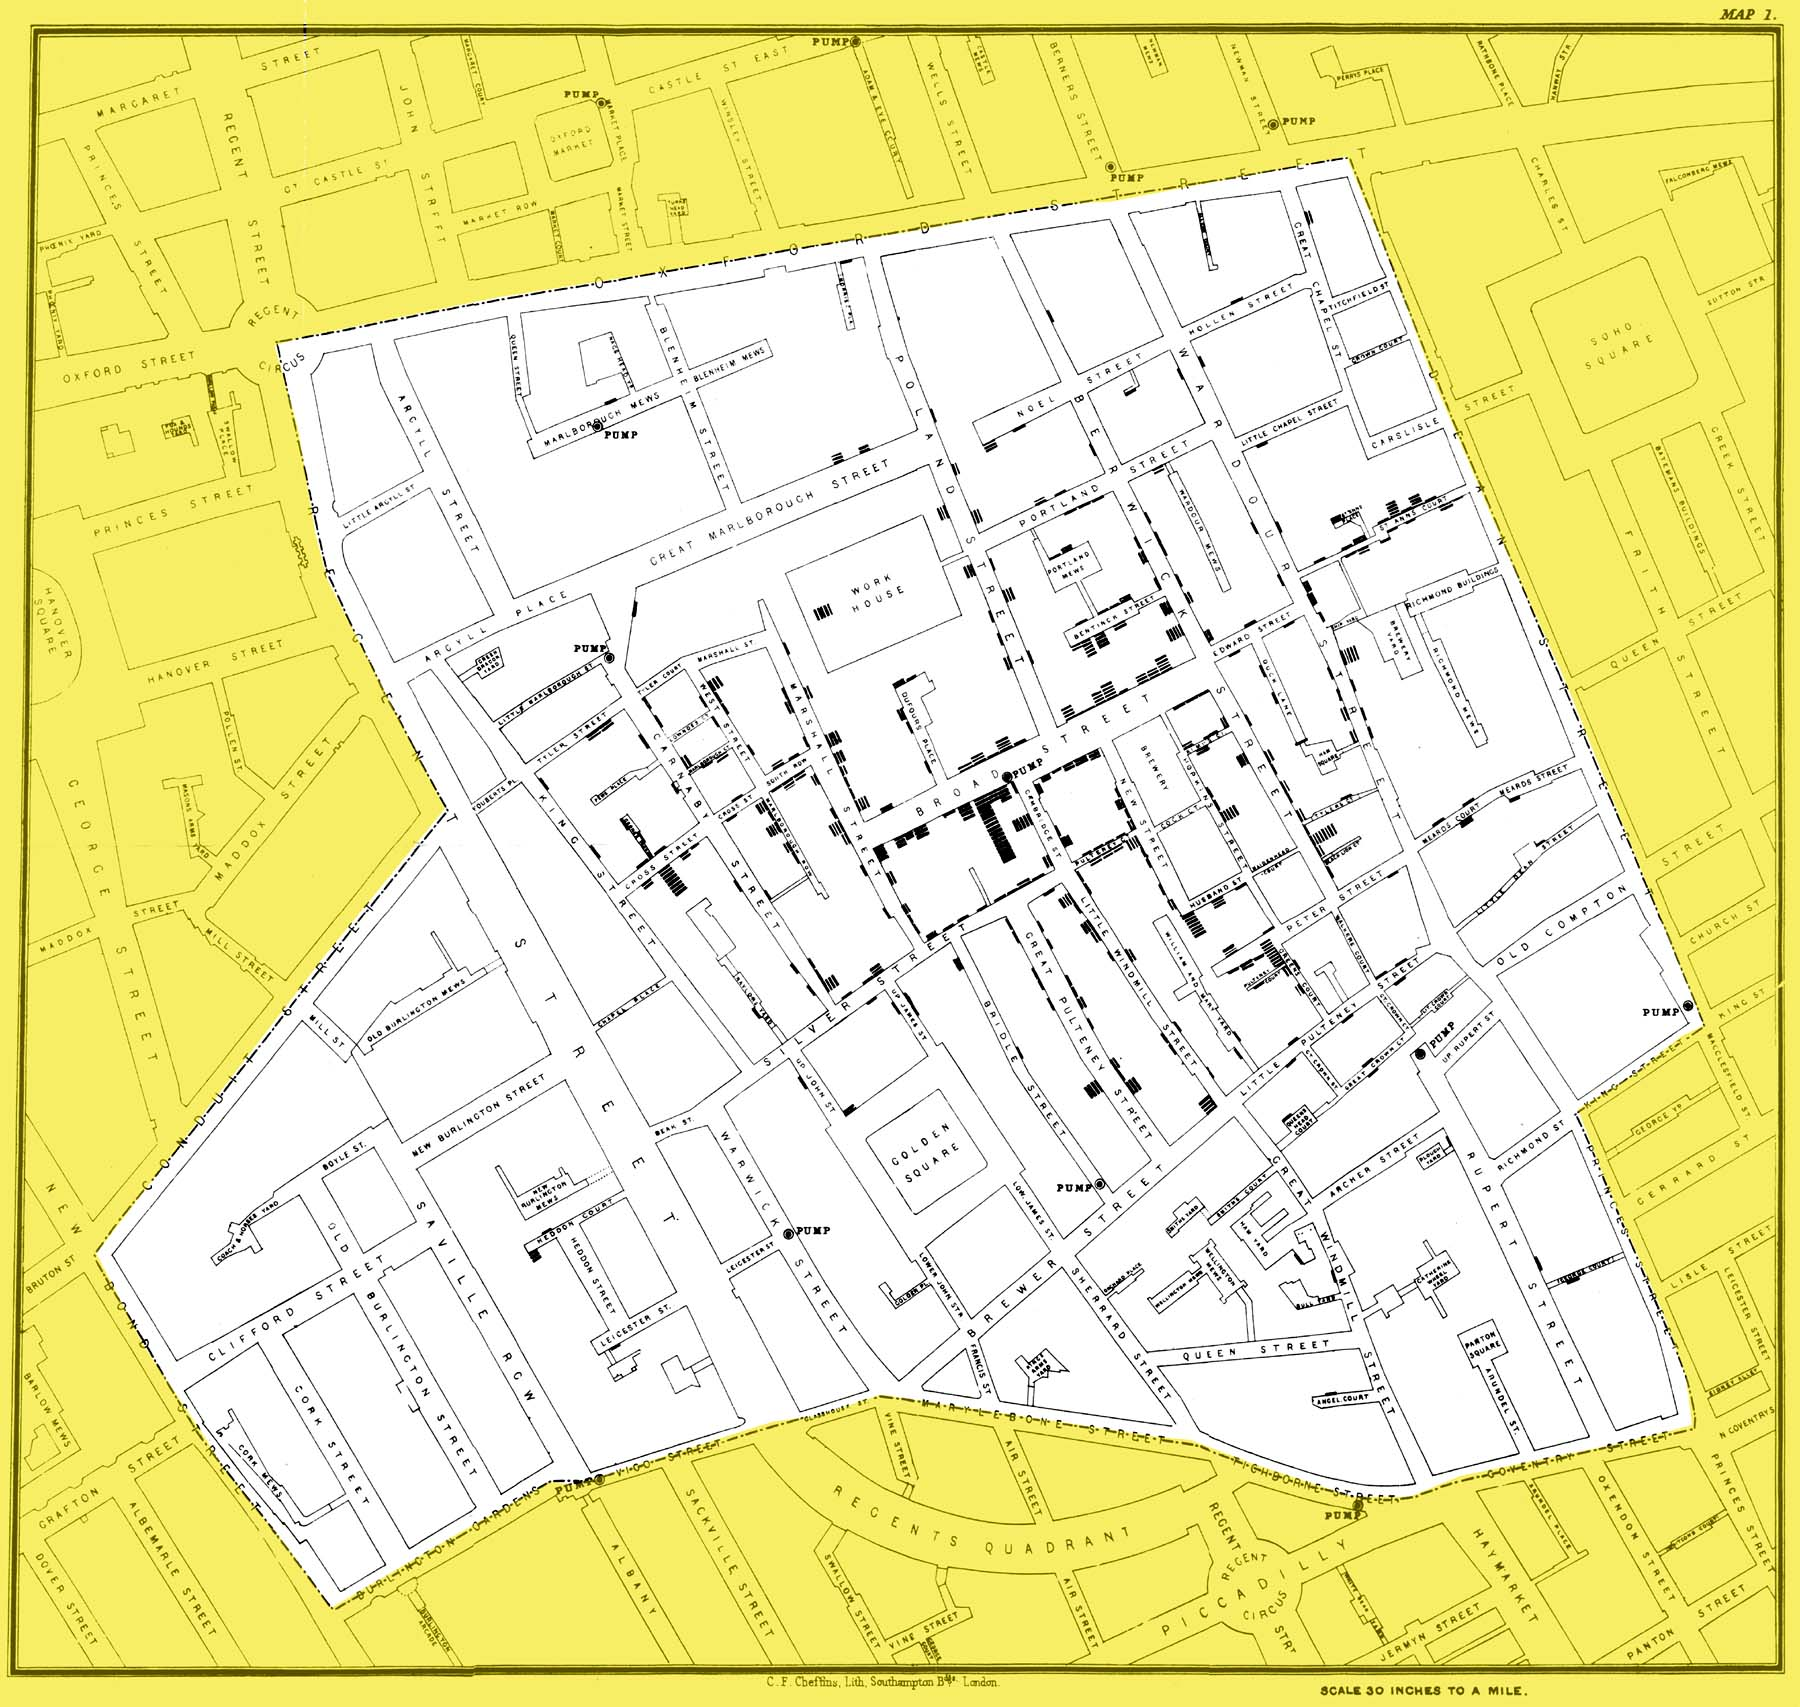
\includegraphics{snowmap_1854}
\caption{Caption}
\label{fig:snow}
\end{figure}

\begin{figure}
\centering
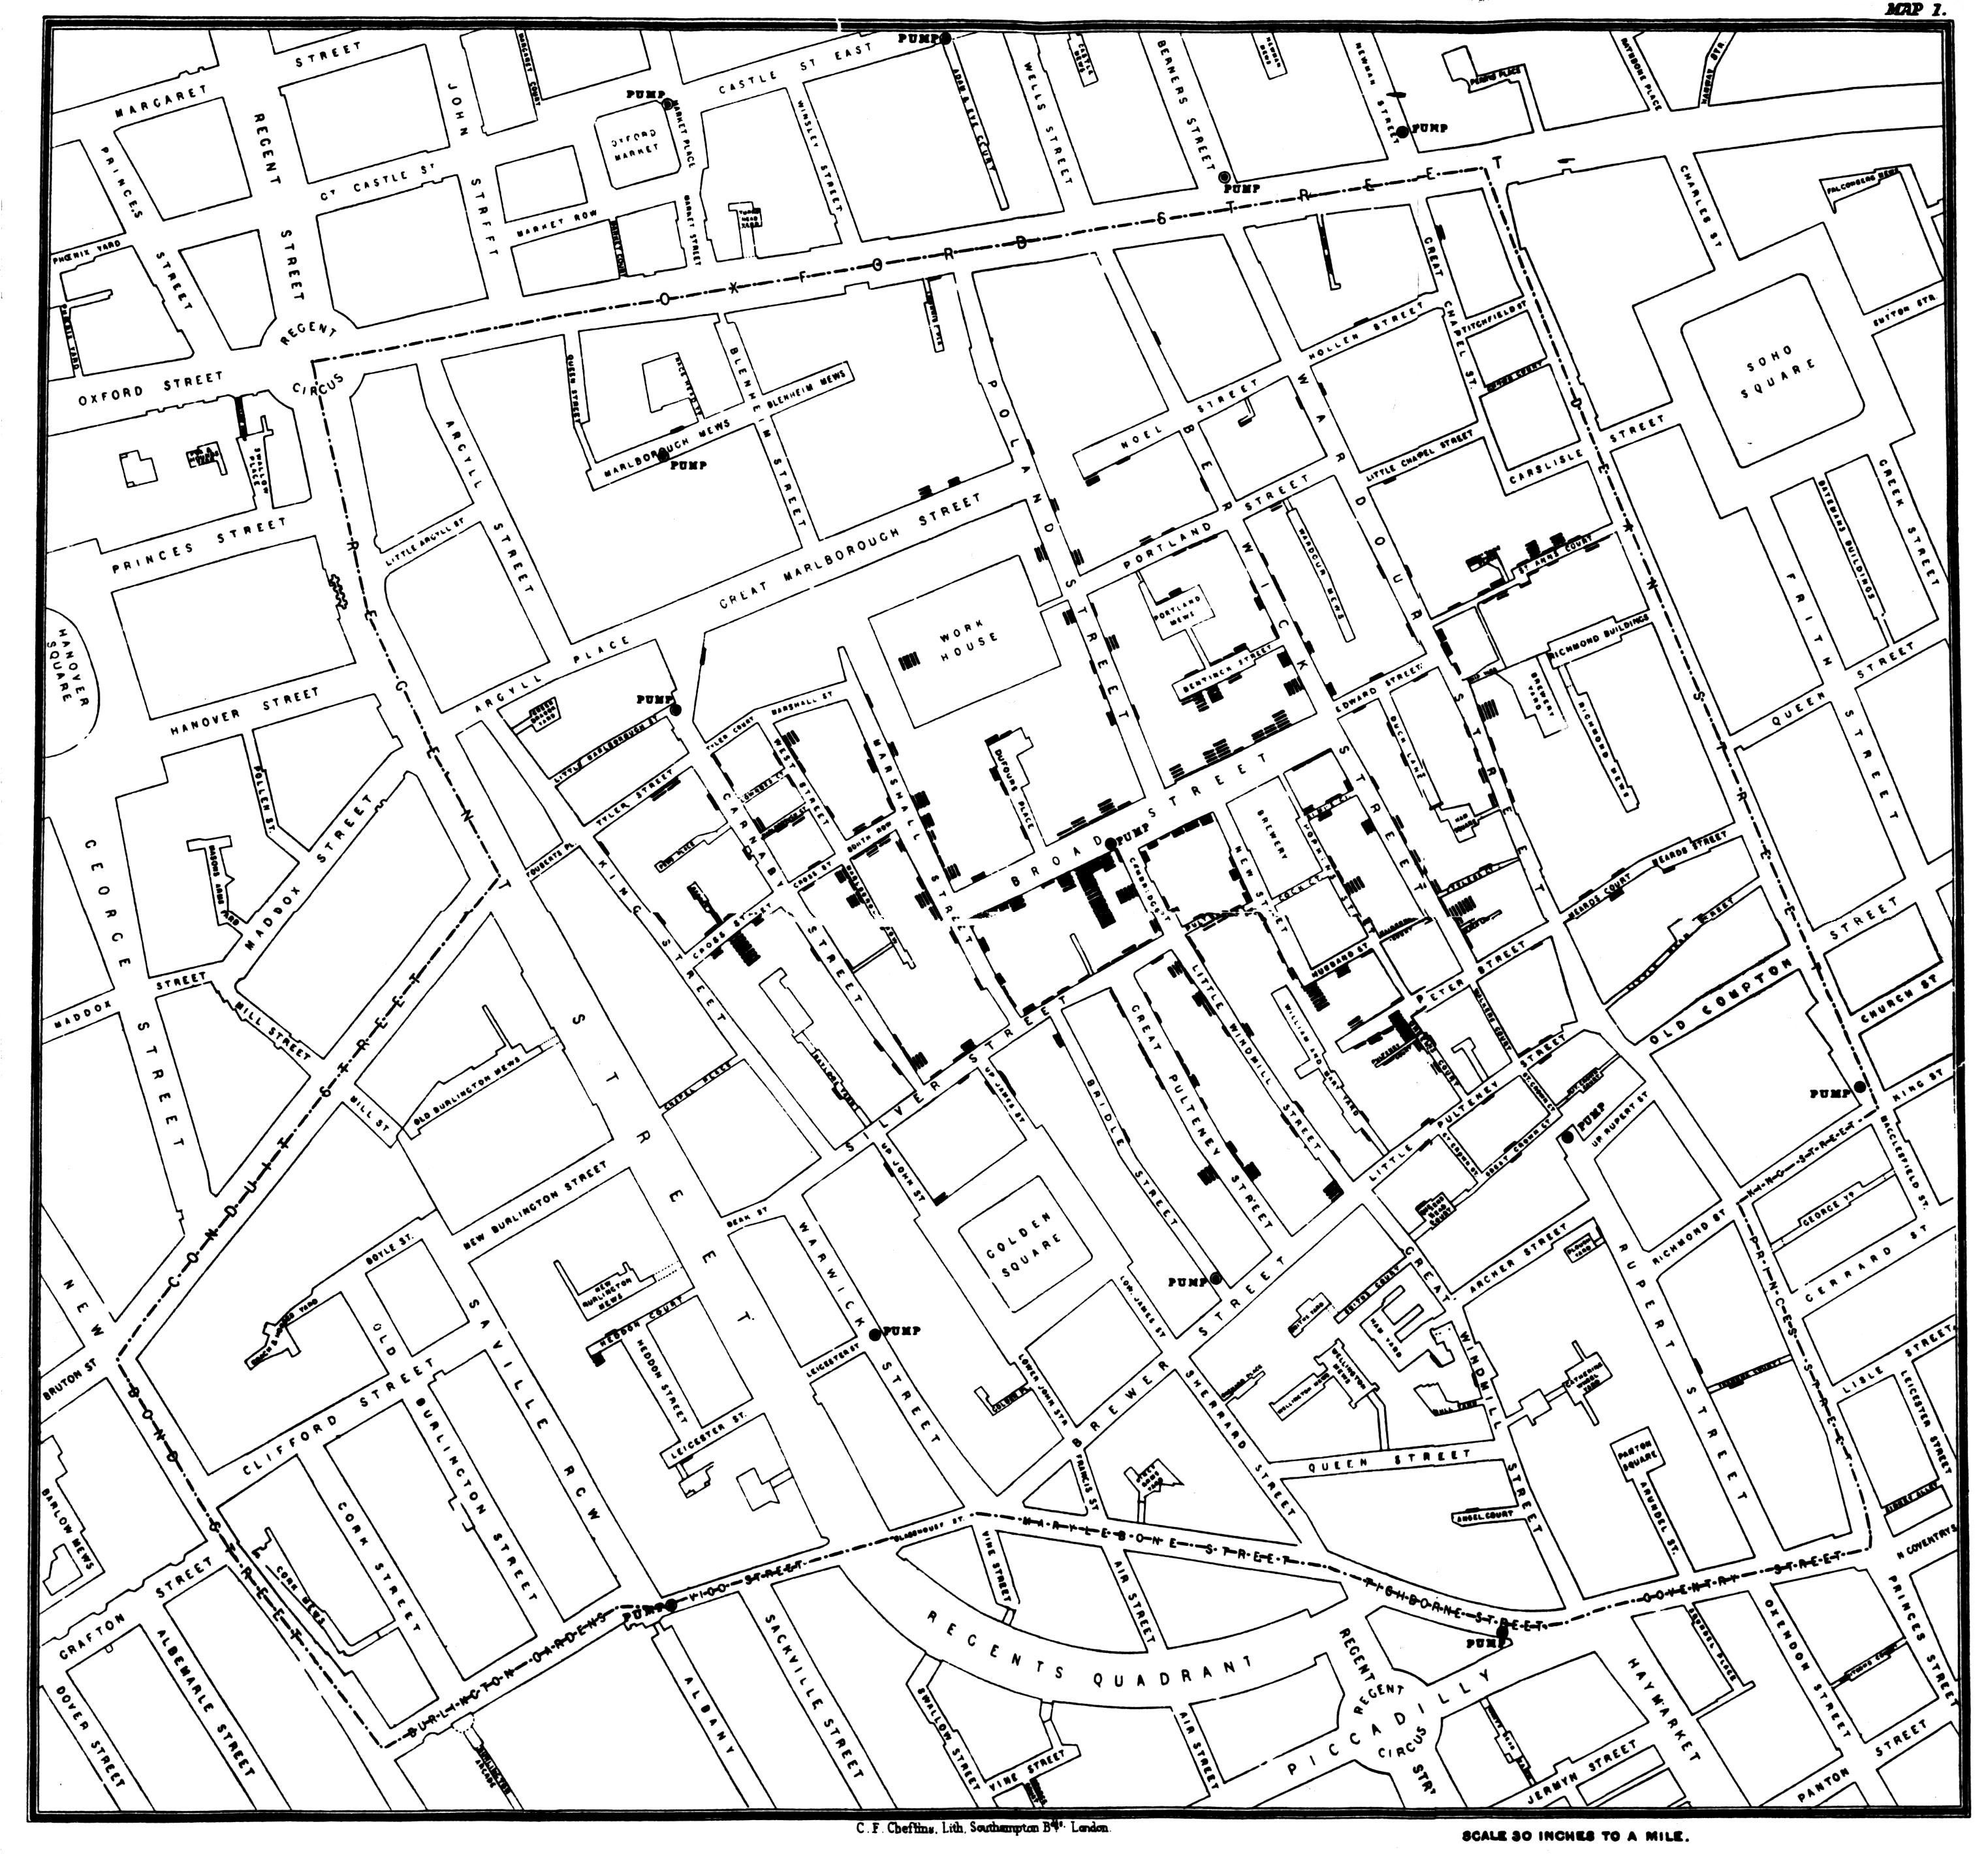
\includegraphics[scale=0.1]{Snow-cholera-map-1}
\caption{John Snow's Cholera map}
\label{fig:snow}
\end{figure}



\section{Weaknesses}

Edward Tufte, a godfather of information display, analyzes this map in his 1997 book, Visual Explanations. Tufte points out that as a dot map, 2 Snow’s visualization is implicitly assuming that the population in the area is uniformly distributed. In other words, a house without any deaths means that the inhabitants of that house successfully avoided cholera, not that the house sits empty. But even with that shortcoming, Tufte praises the map’s usefulness. \cite{blog}

\section{The Impact/Significance/Influence of Snow's Cholera Map}

John Snow's method of mapping the spread of disease is still used today. It was a very clear and scientific approach to taking information, connecting the dots and making sense of what was happening. All the information was out there, but until John Snow, we hadn't put the pieces together yet. \cite{channel1}

When he got authorities to remove the handle, it was more symbolic since the Cholera epidemic had pretty much burnt itself anyway. The real significance of John Snow's story was that its the birth of epidemiology, the birth of statistical analysis, and it shows how many lives you can save, improve conditions with proper conditional surveys. \cite{youtube}

His work addressed an ongoing medical debate — in what is widely regarded as one of the most important early examples of epidemiology, he clearly linked cholera’s spread to water instead of air. \cite{blog}

This map that changed the way the world understood cholera. It forced London to realise it needed to build a sewage system to fix itself and end cholera outbreaks. This map makes my top 5 because it was used to convince people of the need for change. \cite{top5}

His map is not only an important historical moment in public health, but also a breakthrough in the visual display of information. By showing abstract medical statistics within a geographic image, a pattern of illness distribution was made visible in a way that pointed to its cause. Today we call such information visualisations Graphic Information Systems (GIS for short). \cite{test}

Steven Johnson, in his book “The Ghost Map” about the London cholera epidemic and efforts to stop it, notes that Snow’s was not the first map to chronicle cholera outbreaks, or even this particular cholera outbreak. \cite{history}

\section{Similar Visualisations in the nineteenth century}
\todo{could be moved to history?}
Among the earliest examples of disease mapping were
two spot maps prepared by Valentine Seaman to illustrate
the distribution of yellow fever in New York
towards the close of the eighteenth century. Shapter2, in
his History of the Cholera in Exeter in 1832 included a dot
map showing the distribution of deaths caused by
cholera. (Figure 1). \cite{howe1970some}

“Part of what made Snow’s map groundbreaking was the fact that it wedded state-of-the-art information design to a scientifically valid theory of cholera’s transmission. It was not the mapmaking technique that mattered; it was the underlying science that the map revealed,” Johnson writes. \cite{history}

It's possible to solve these problems, if we look at the empirical evidence such as the map. ``It's a  map of deaths that ended up creating a whole new way of life, a life that we are enjoying today." \cite{tedtalk}

\todo{from wikipedia}
Snow's study was a major event in the history of public health and geography. It is regarded as the founding event of the science of epidemiology.


\section{Modern Visualisations}

\section{Conclusion}


% \bibliographystyle{IEEEtranN}
% \bibliographystyle{ieeetr}


\bibliography{mybib}
\bibliographystyle{ieeetr}

\end{document}